\documentclass{article}

% if you need to pass options to natbib, use, e.g.:
\PassOptionsToPackage{numbers, compress}{natbib}
% before loading nips_2018

% ready for submission
\usepackage[final]{nips_2018}

% to compile a preprint version, e.g., for submission to arXiv, add
% add the [preprint] option:
% \usepackage[preprint]{nips_2018}

% to compile a camera-ready version, add the [final] option, e.g.:
% \usepackage[final]{nips_2018}

% to avoid loading the natbib package, add option nonatbib:
% \usepackage[nonatbib]{nips_2018}

\usepackage[utf8]{inputenc} % allow utf-8 input
\usepackage[T1]{fontenc}    % use 8-bit T1 fonts
\usepackage{hyperref}       % hyperlinks
\usepackage{url}            % simple URL typesetting
\usepackage{booktabs}       % professional-quality tables
\usepackage{amsfonts}       % blackboard math symbols
\usepackage{nicefrac}       % compact symbols for 1/2, etc.
\usepackage{microtype}      % microtypography
\usepackage{graphicx}

\title{How Are You Feeling? \\ Inferring Mood from Audio Samples}


% The \author macro works with any number of authors. There are two
% commands used to separate the names and addresses of multiple
% authors: \And and \AND.
%
% Using \And between authors leaves it to LaTeX to determine where to
% break the lines. Using \AND forces a line break at that point. So,
% if LaTeX puts 3 of 4 authors names on the first line, and the last
% on the second line, try using \AND instead of \And before the third
% author name.

\author{
  Joel Haynie \\
  Department of Computer Sciences\\
  University of Wisconsin, Madison\\
  \texttt{email@wisc.edu} \\
  \And
  Ankit Vij \\
  Department of Computer Sciences\\
  University of Wisconsin, Madison\\
  \texttt{email@wisc.edu} \\
  \AND
  Amanpreet Singh Saini \\
  Department of Computer Sciences\\
  University of Wisconsin, Madison\\
  \texttt{email@wisc.edu} \\
  \And
  Eric Brandt \\
  Department of Computer Sciences\\
  University of Wisconsin, Madison\\
  \texttt{ebrandt@wisc.edu}
}

\begin{document}
% \nipsfinalcopy is no longer used

\maketitle

\begin{abstract}
  The abstract paragraph should be indented \nicefrac{1}{2}~inch
  (3~picas) on both the left- and right-hand margins. Use 10~point
  type, with a vertical spacing (leading) of 11~points.  The word
  \textbf{Abstract} must be centered, bold, and in point size 12. Two
  line spaces precede the abstract. The abstract must be limited to
  one paragraph.
\end{abstract}

\section{Background}

Works we plan to cite (to make sure bibtex is working): 
\begin{itemize}
\item CNN Architectures for Large-Scale Audio Classification, Hershey\cite{hershey}
\item What’s wrong with CNNs and spectrograms for audio processing?, Rothmann\cite{rothmann}
\item Inside the spectrogram: Convolutional Neural Networks in audio processing, Dorfler\cite{dorfler}
\item Getting Started with Audio Data Analysis using Deep Learning, Shaikh\cite{shaikh}
\item Hearing AI: Getting Started with Deep Learning for Audio on Azure, Zhu\cite{zhu}
\item How do deep convolutional neural networks learn from raw audio waveforms?, Gong\cite{gong}
\item AudioSet \cite{audioset}
\item TensorFlow \cite{tensorflow}
\item Keras \cite{keras}
\end{itemize}
	
\section{Implementation}

\subsection{Data Acquisition and Extraction}

We collected our data from Google’s AudioSet \cite{audioset} which consists of an expanding ontology of 632 audio event classes and a collection of 2,084,320 human-labeled 10-second sound clips drawn from YouTube videos. The ontology is specified as a hierarchical graph of event categories, covering a wide range of human and animal sounds, musical instruments and genres, and common everyday environmental sounds. From the dataset, we focussed on music mood samples and extracted data points with 4 mood classes- Happy, Sad, Angry, and Scary. The dataset had two groups, `unbalanced' and `evaluation' set (We used the `unbalanced' data set because the `balanced' data set was too small for our needs). We created a \texttt{.csv} of 223 data points with their labels from the `evaluation' set with \~56 entries for each mood class. Additionally, we created a \texttt{.csv} of 400 data points with their labels from the `unbalanced' set with 100 entries for each mood class. These CSVs were then used to for two purposes:
\begin{enumerate}
\item Download the corresponding Google-produced spectrographs of each of the samples for use in establishing a baseline classification accuracy.
\item Download the audio samples in .WAV format directly from their source (YouTube) which we used in the pre-processing step described in the next section.
\end{enumerate}


\subsection{Baseline}

To establish a baseline for the achievable accuracy in learning a  multi-class classification task, we began by using the spectrographs for the 400 + 223 data instances we identified as a) being music audio, and b) having one of the 4 mood labels we chose for analysis.

To evaluate this baseline, Python was used, enlisting the libraries TensorFlow \cite{tensorflow} and Keras \cite{keras}.

The 400 samples were evenly divided by class for stratified k-fold cross validation and used to train 3 different neural networks:
\begin{enumerate}
\item Simple multi-class logistic regression classifier
\item 1-Layer LSTM (Long-short term memory) recurrent neural network
\item 3-Layer LSTM (Long-short term memory) recurrent neural network
\end{enumerate}
In each case, the model was trained using batches of 40 samples, randomized at each presentation, for a sufficient number of epochs to infer steady-state accuracy.

We evaluated the performance of each of the 3 models by two methods:
\begin{enumerate}
\item Validation set accuracy over an increasing number of epochs.
\item Evaluation on a Test Set of 223 never-seen-before data instances (\texttt{audioset/eval}).
\end{enumerate}

The performance of the training sessions is shown in figure \ref{fig:baseline_train}.
\begin{figure}[]
	\centering
	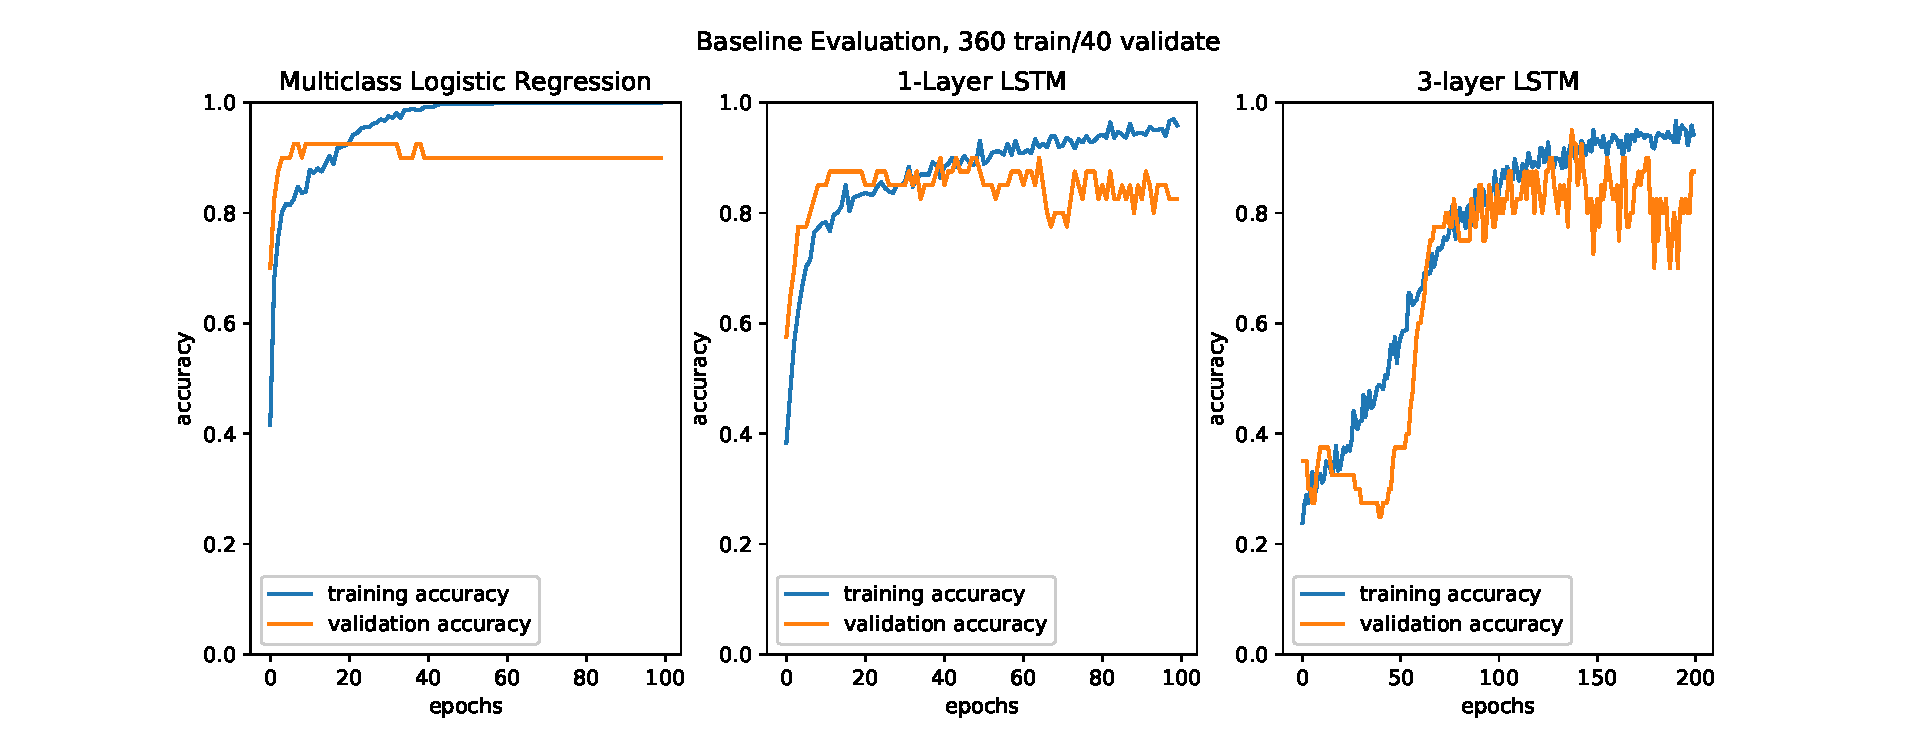
\includegraphics[width=1.25\textwidth]{Baseline400.eps}  
	\caption{Baseline training performance for 3 models.}
	\label{fig:baseline_train}
\end{figure}

After training, the evaluation on  the 220-instance balanced test set, we observed the accuracies shown in table \ref{tbl:baseline_acc}.
\begin{table}[] 
\caption{Baseline accuracy on held-aside test set of 220 instances for 3 models.}
\label{tbl:baseline_acc}
\centering
\begin{tabular}{lc} 
\toprule
\hline
Model & Accuracy \\ 
\midrule
Logistic Regression & 0.803 \\
1-Layer LSTM & 0.830 \\ 
3-Layer LSTM & 0.731 \\ 
\bottomrule
\end{tabular}
\end{table}

Finally, to make sure that our four chosen classes do not have an abnormal correlation between any combinations of classes, we also computed confusion matrices for the models. The confusion matrix for Logistic Regression (arguably the best performing classifier) is shown in table \ref{tbl:baseline_conf}.

\begin{table}[] 
\caption{Confusion matrix for baseline logistic regression classifier of 223 test instances.}
\label{tbl:baseline_conf}
\centering
\begin{tabular}{lcccc} 
\toprule
\hline
 & Happy & Sad & Angry & Scary \\ 
\midrule
Happy & 45 &  9 & 2 & 1 \\
Sad   &  11 & 39 & 2 & 4 \\
Angry &  0 &  1 & 53 & 4 \\
Scary &  0 &  7 & 3 &  42 \\
\bottomrule
\end{tabular}
\end{table}

From the baseline evaluation we can draw some conclusions and inferences:
\begin{itemize}
\item The input feature sets must be nearly linearly separable, as evidenced by the strong performance of the simple multiclass logistic regression classifier.
\item Google’s preprocessing of the raw audio waveforms into 10-frame spectrographs, including processing by Google’s own CNN and PCA reduction clearly has produced data that is well separated without significant further processing.
\item Evidence of the linearly separable feature data is supported by much more complicated non-linear classifiers (1-Layer LSTM and 3-Layer LSTM) not yielding better performance.
\item There is evidence that the LSTM models are subject to overtraining at higher numbers of epochs.
\item More complicated models with more parameters, particularly the 3-Layer LSTM, take significantly more time to train.
\item The confusion matrix suggests, surprisingly, that ‘Happy’ and ‘Sad’ are the most often confused classifications, and that ‘Scary’ and ‘Angry’ are comparatively easy to predict.
\end{itemize}


\subsection{Preprocessing}

\subsection{CNN Training}

\section{Discussion}

\section{Conclusion}

\subsection{Future Work}
  
\bibliography{Bibliography} 
\bibliographystyle{plainnat}

\end{document}
